\documentclass{zcu_sp}
\usepackage[utf8]{inputenc}
\usepackage[czech]{babel}
\usepackage{amsmath}
\usepackage{graphicx}

\usepackage[pdfborder=0 0 0]{hyperref}



\title{Pohoda na Sahaře}
\course{KIV/ZPG}
\author{Tomáš Maršálek}
\email{marsalet@students.zcu.cz}
\date{14.\,prosince 2012}



\begin{document}
\maketitle
\section{Úvod}
Pro semestrální práci jsem po osobní dohodě se cvičícím zvolil jazyk Java, poté
podle vlastního výběru jeden z nejpoužívanějších wrapperů OpenGL pro Javu -
\textbf {Lightweight Java Game Library (LWJGL)}.

\section{Pohyb po terénu}
\subsection{Rychlostní vektor}
Požadavkem je, aby rychlost pohybu hráče po terénu byla konstantní ve všech
směrech. Postup, který je zde použit nejprve vytvoří rychlostní vektor v rovině
xz, které zjistí ze stisknutých kláves WSAD. Současná pozice s tímto vektorem
udává novou pozici. Nad ní je doplněna výšková souřadnice a rychlostní vektor
je normalizován. Problém, který nastane, je ten, že po normalizaci vznikla
chyba ve výškové složce rychlostního vektoru. Proto je souřadnice y vypočítána
znovu a vektor opět normalizován. Tento postup je iterován, dokud není dosaženo
přijatelné chyby. Tato metoda obecně nekonverguje, proto je počet iterací
omezen konečnou hodnotou.

\subsection{Fyzika}
Jsou implementována dvě rozšíření nad standardním pohybem. Jedním z nich je implementace setrvačnosti po zvednutí pohybových kláves. V každém snímku je pouze rychlostní vektor přenásoben útlumovou konstantou $c, 0 < c < 1$.

Druhým rozšířením je skok do výšky. Vektor rychlosti je ve finále počítán jako
součet vektoru rychlosti vypočteném podle stisknutých pohybových kláves,
vektoru skoku a vektoru představujícího gravitaci.
\begin{align*}
\mathbf{v} = \mathbf{velocity}+ \mathbf{jump} - gravityConstant \cdot t \\
\end{align*}

Po získání vektoru rychlosti získáme pozici hráče v novém snímku ze vztahu
$\mathbf{s} = \mathbf{v} \cdot t$
Čas $t$ je zde časový rozdíl mezi snímky.

\subsection{Detekce kolizí}
Kolize s terénem jsou vypočteny jednoduše jako 
\begin{align*}
y &:= max(y, getY(x, z))
\end{align*}


\section{Terén}
Terén je načten z raw souboru, který reprezentuje výškovou mapu pro každý z
bodů roviny xz. Tyto řídící body jsou uloženy do dvourozměrného pole bodů $h$.
Terén je pak v programu reprezentován funkcí $getY(x, z) = y$, která používá
body výškové mapy a interpoluje ty body, které leží mezi řídícími.V

\subsection{getY}
Pro funkci getY můžeme použít nespojitou funkci \uv{schody}. Tj. $getY(x, z) =
h (\lfloor x \rfloor, \lfloor z \rfloor)$.

\subsubsection{Bilineární interpolace}
Lepší řešení poskytuje použití spojité interpolace. Protože se jedná o
interpolaci ve dvou rozměrech, uvažujeme interpolaci bilineární.

Její princip spočívá ve dvojité lineární interpolaci mezi čtyřmi body A, B, C,
D, když máme zadány interpolační koeficienty $u$ a $v$ pro každý ze dvou
rozměrů. Nejprve najdeme pomocné body, které leží na přímkách mezi body A a B,
respektive C a D.
\begin{align*}
E &= linearInterpolate(A, B, u) \\
F &= linearInterpolate(C, D, u) \\
\end{align*}
Nakonec proložíme přímku mezi těmito body, čímž podruhé použijeme lineární interpolaci - odtud název metody.
\begin{align*}
G &= linearInterpolate(E, F, v) \\
\end{align*}

\subsubsection{Bilinearly blended patch}
Pokud chceme nejen spojitou funkci, ale i spojitou derivaci, tzn. aby se na
povrchu netvořily špičaté vrcholy, musíme použít funkci se spojitou první
derivací. Pro dosažení vyhlazeného povrchu se nejčastěji používá bikubická nebo
bilineární interpolace mezi kubickými křivkami mezi řídícími vrcholy. Zde byla
zvolena bilineárně namíchaná interpolace (bilinearly blended patch) mezi
Catmull-Rom spline křivkami. Použití bikubické interpolace namísto bilineární
nepřináší znatelně více hladkosti, více záleží na kontrolních křivkách.

Catmull-Rom spline je hladká interpolační křivka mezi n body, která je často
používána pro svou jednoduchost. Pro výpočet používá Hermittovu formu kubické spline křivky, kde parametry derivace jsou zvoleny pro sousední body shodné, aby došlo právě ke kýžené hladkosti.

Lepším řešením by bylo použití b-spline křivky, která dosahuje spojité i druhé
derivace, za cenu složitějšího výpočtu.

Bilinearly blended patch je metoda pro získání bodu, který se nachází na povrchu ohraničeném čtyřmi libovolnými křivkami.
Nejprve jsou spočteny body na kontrolních křivkách dle parametrů u a v. 
\begin{align*}
E &= spline(A, B, u) \\
F &= spline(C, D, u) \\
G &= spline(A, C, v) \\
H &= spline(B, D, v) \\
\end{align*}
Tyto jsou lineárně interpolovány
\begin{align*}
I &= linearInterpolate(E, F, v) \\
J &= linearInterpolate(G, H, u) \\
\end{align*}

Výsledek je součet těchto dvou lineárních interpolací, od kterých je odečtena jedna bilineární interpolace:
\begin{align*}
K &= I + J - bilinearInterpolate(A, B, C, D, u, v) \\
\end{align*}

\begin{figure}[ht!]
\centering
	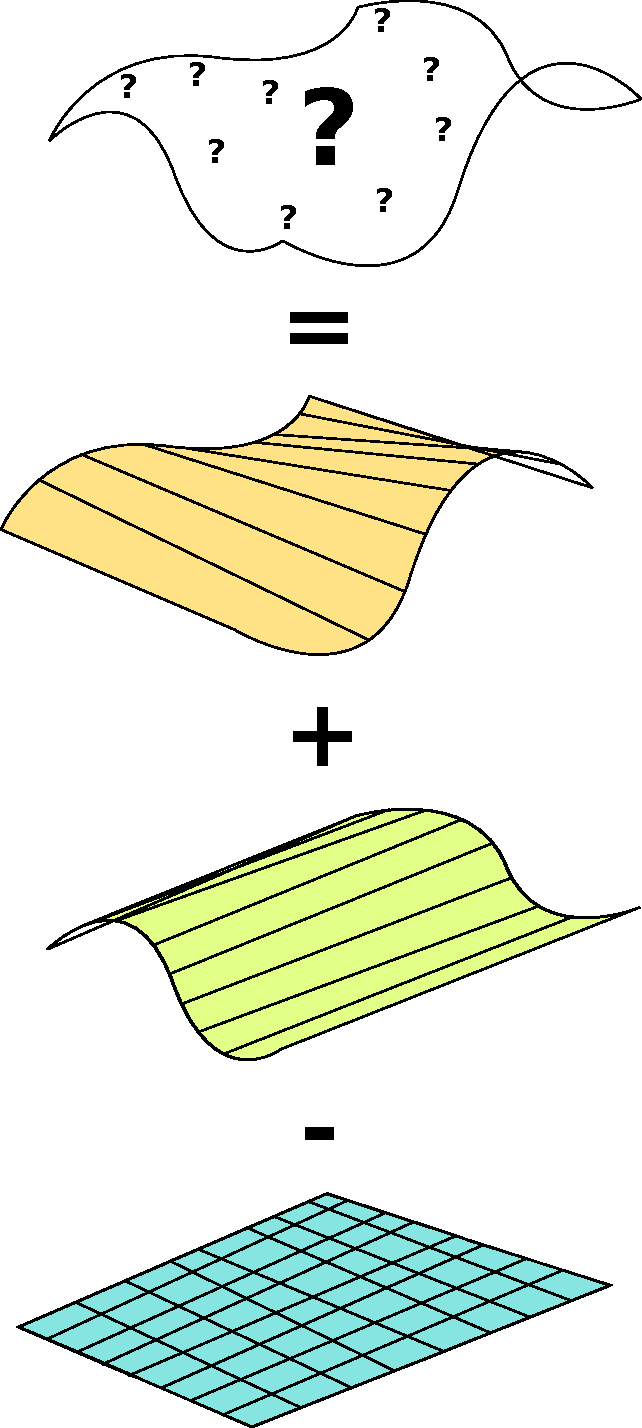
\includegraphics[width=8cm]{coons.pdf}
	\caption{Bilinearly blended patch mezi čtyřmi kontrolními křivkami.}
\end{figure}


\subsection{Vyhlazování}
Pro vykreslování je terén uložen do vertex bufferu na grafické kartě. Na
základě úrovně rozdělení je terén opakovaně rozčtvrcen a nově vzniklé body
určené podle zvolené interpolující funkce.


\subsection{Adaptivní vyhlazování}
Terén, který je zadán jako výšková mapa velikosti $128\times128$, je po
zjemnění úrovně 3 velký $1024\times1024$. Vykreslování takto detailního terénu
je výpočetně zbytečně složité, proto se úroveň vyhlazování (LOD - Level of
Detail) určujeme na základě vzdálenosti od pozorovatele. Čím blíže, tím
očekáváme detailnější terén a naopak. 

\subsection{Quadtree}
Datová struktura, ve které je uložená reprezentace vyhlazeného povrchu je
Quadtree. Její největší přínos je snadná teselace terénu, zejména tam, kde na
sebe navazují rozdílné úrovně vyhlazení.

Quadtree je stromová struktura, jejíž kořenový uzel představuje celý terén jako
jeden čtyřúhelník. Potomci tohoto a každého dalšího uzlu jsou čtyři čtvrtiny
tohoto čtyřúhelníka, respektive čtyřúhelníka, který daný uzel představuje.

Při vykreslování každého snímku je tento strom rozložen do požadované
hloubky a na konci opět složen zpátky. Obě operace jsou rekurzivní,
jedna úroveň vytvoření potomků vypadá takto:


\begin{figure}[ht!]
\centering
	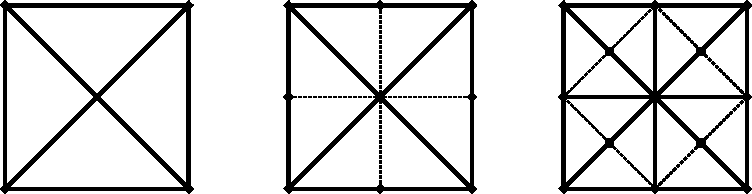
\includegraphics[width=10cm]{subd.pdf}
	\caption{Vytvoření potomků uzlu.}
\end{figure}

\begin{figure}[ht!]
\centering
	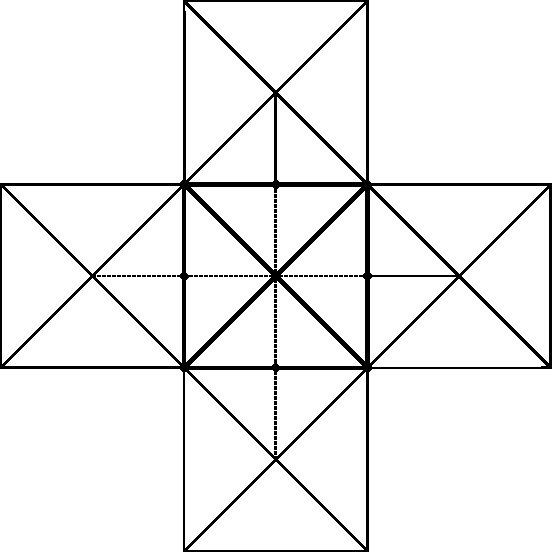
\includegraphics[width=8cm]{split.pdf}
	\caption{Rozložení uzlu a korekce u sousedních uzlů.}
\end{figure}
Složení je pak pouze opačná operace.

Popis a implementace Quadtree pro adaptivní vyhlazování je delailněji a lépe popsán v několika publikacích a článcích. % TODO cite quadtree

\subsection{Výpočet normály}
Při ukládání vrcholů do vertex bufferu jsou zároveň spočteny normály pro každý
bod. Metoda spočívá ve výpočtu gradientu takové funkce, že terén, tedy $getY(x,
z)$, je jednou z jejích vrstevnic. Pro vektor gradientu platí, že je vždy kolmý
na vrstevnici své křivky, což je přesně to, co potřebujeme pro normálu.

Funkce, kterou hledáme je $f(x, y, z) = getY(x, z) - y$, protože $c = getY(x,
z) - y$ je obecný předpis pro vrstevnici $f$ a pro $c = 0$ dostáváme náš terén. 
Gradient této funkce je jednoduše
\begin{align*}
\nabla f = \left[ \frac{\partial getY}{\partial x}, -1, \frac{\partial getY}{\partial z} \right]^T
\end{align*}

Derivaci samozřejmě spočteme numericky, například pomocí obousměrné diference.
Gradient normalizujeme a máme jednotkový vektor normály pro daný bod.


\section{Pohledové ořezávání}
Počet trojúhelníků, které budeme chtít vykreslit nebo vyhladit pomocí quadtree, můžeme výrazně omezit tak, že vynecháme všechny uzly, které se ve výsledném snímku vůbec nezobrazí.

Provedeme vlastně clipping, tedy oříznutí elementů mimo snímek, stejně jako ho
za nás provede OpenGL ve výsledném snímku. Abychom mohli tuto proceduru
aplikovat, musíme získat projekční a modelview matici, se kterými v daném
snímku grafická knihovna pracuje.

Pro převedení souřadnic bodu $\mathbf{b}$ z modelových do clipping souřadnic
použijeme modelview $\mathbf{M}$ a projekční matici $\mathbf{P}$:
\begin{align*}
\mathbf{b_{world}} &= \mathbf{M} \mathbf{b} \\
\mathbf{b_{clip}} &= \mathbf{P} \mathbf{b_{world}} \\
\mathbf{b_{clip}} &= \mathbf{P} \mathbf{M} \mathbf{b} \\
\end{align*}

Ve skutečnosti nás zajímá matice pro převod z modelových do clipping souřadnic, tedy součin modelview a projekční matice. Její řádky se poté použijí pro konstrukci stěn komolého jehlanu (view frustum), který představuje viditelnou oblast.
\begin{align*}
\begin{pmatrix}x\\y\\z\\w\end{pmatrix} = \mathbf{PM} \mathbf{b} = \begin{pmatrix}pm_1^T\\pm_2^T\\pm_3^T\\pm_4^T\end{pmatrix} \mathbf{b}\\
\end{align*}

V clipping souřadnicích je snadné určit, zda se bod $\mathbf{b_{clip}} = \left[
x, y, z, w \right]^T$ nachází uvnitř pohledové pyramidy, či nikoliv. Bod uvnitř splňuje šest nerovnic, pro každou z šesti stran komolé pyramidy.
\begin{align*}
-w \leq & x \leq w \\
-w \leq & y \leq w \\
-w \leq & z \leq w \\
\end{align*}

Protože ale $w$ je reprezentován posledním řádkem $pm_4^T \mathbf{b}$ a $x$ je $pm_1^T \mathbf{b}$, přepíšeme první nerovnici:
\begin{align*}
-pm_4^T \mathbf{b} &\leq pm_1^T \mathbf{b} \\ 
0 &\leq pm_1^T \mathbf{b} + pm_4^T \mathbf{b} \\
0 &\leq (pm_1^T + pm_4^T) \mathbf{b} \\
\end{align*}

Poslední rovnice představuje rovnici první roviny pohledové pyramidy. Stejným způsobem zjistíme zbylých pět. 







\section{Osvětlení}
\subsection{Plynulá intenzita světla}
Máme-li den, který trvá od času 0 (00:00) do 1 (24:00), očekáváme v čase 0.5
nejvyšší intenzitu světla. Použitá funkce určující intenzitu slunce je Gaussova
křivka centrovaná do bodu 0.5.
$$
Intenzita~=~e^{- (C(t - \frac{1}{2}))^2}
$$
kde C je magická konstanta, která byla nalezena po chvíli testování tak, aby
byl výsledek co nejbližší skutečnosti.

Získaná intenzita se používá přímo jako intenzita hlavního zdroje světla - slunce a jako barva atmosféry.
\subsection{Ambientní osvětlení}
Scénu navíc osvětluje globální ambientní iluminace a dvě světla umístěná nad
dvěma protilehlými rohy terénu, která vrhají realistický stín i v "noci".

\section{Přehled implementovaných variací}
\begin{itemize}
	\item grafický vzhled a efekty
	\begin{itemize}
		\item pohledové ořezávání pyramidou
		\item hladký terén
		\item adaptivní zjemňování terénu
	\end{itemize}

	\item avatar, uživatelské rozhranní a pomoc hráči
	\begin{itemize}
		\item dynamika avatara (hráče)
	\end{itemize}
\end{itemize}

\section{Přeložení a spuštění}
\section{Ovládání hry}
Kamerou pohneme standardně klávesami WSAD nebo šipkami a otočíme pohybem myši.
Skok je pomocí mezerníku. Invertování vertikálního pohledu provedeme pomocí
klávesy U a přepnutí mezi drátěným a plným modelem pomocí klávesy C. Hru
ukončíme stiskem klávesy ESC.

\section{Závěr}
Výsledkem je spíše jednoduchý základ pro hru, než hra samotná. Zaměřil jsem se
především na výpočetně orientované variace úlohy. I přesto, že se jedná o pouhý
terén a pohyb po něm, jedním jednoduchým vylepšením scény by bylo otexturování
terénu na základě například výšky nebo sklonu v daném bodě.

Dále jsem chtěl implementovat vyhlazování pomocí kubické b-spline křivky a
porovnat s hotovou Catmull-Rom křivkou. 


\begin{thebibliography}{5}
\bibitem[1]{rocks}
{\em Bill Jacobs} \\
{\bf OpenGL tutorial}
	2007 - 2012 \\
\url{http://www.videotutorialsrock.com/}

\bibitem[2]{installtut}
{\em TheCodingUniverse} \\
{\bf \#1 LWJGL Workspace - LWJGL Tutorials} \\
	2011 \\
\url{http://youtu.be/0v56I5UWrYY}

\bibitem[3]{wikistrips}
{\em Wikipedia contributors} \\
{\bf ``Triangle strip,'' Wikipedia, The Free Encyclopedia} \\
	(accessed October 27, 2012) \\
\url{http://en.wikipedia.org/wiki/Triangle_strip}

\bibitem[4]{wikicoons}
{\em Wikipedia contributors} \\
{\bf ``Coons surface,'' Wikipedia, The Free Encyclopedia} \\
	(accessed 14 December 2012) \\
\url{http://en.wikipedia.org/w/index.php?title=Coons_surface&oldid=486532739}

\bibitem[5]{rygblogFrustum}
{\em The ryg blog} \\
{\bf Frustum planes from the projection matrix} \\
\url{http://fgiesen.wordpress.com/2012/08/31/frustum-planes-from-the-projection-matrix/}

\bibitem[6]{flipcodeFrustum}
{\em Dion Picco - flipcode} \\
{\bf Frustum Culling} \\
\url{http://www.flipcode.com/archives/Frustum_Culling.shtml}

\bibitem[7]{xna-large-terrain}
{\em skytiger} \\
{\bf XNA Large Terrain} \\
\url{http://skytiger.wordpress.com/2010/11/28/xna-large-terrain/}

\bibitem[8]{xna-terrain-tutorial}
{\em Dustin Horne} \\
{\bf XNA Terrain Tutorial} \\
\url{http://www.dustinhorne.com/page/XNA-Terrain-Tutorial-Table-of-Contents.aspx}

\bibitem[9]{rose-hulman}
{\em David L. Finn} \\
{\bf MA 323 Geometric Modelling \\ Course Notes: Day 31 \\ Blended and Ruled Surfaces Coons Patches} \\
\url{http://www.rose-hulman.edu/~finn/CCLI/Notes/day31.pdf}

\end{thebibliography}

\end{document}
